\documentclass{article}
\usepackage{amsmath}
\usepackage{upgreek}
\usepackage{dsfont}
\usepackage{mdframed}
%margin package
\usepackage[margin=1in,includefoot]{geometry}
%graphics packages
\usepackage{graphicx}
\usepackage{float}
%pseudocode packages
\usepackage{amsmath}
\usepackage{algorithm}
\usepackage[noend]{algpseudocode}
%hyperlinks
\usepackage{hyperref}

\begin{document}

\begin{titlepage}
	\begin{center}
	\line(1,0){400}\\
	\huge{\bfseries Second report on the paper "Iterated Tabu Search and 		Variable Neighborhood Descend for packing unequal circles into a circular container".}\\
	\line(1,0){400}\\
	\textsc{\Large About the implemented algorithms }
	\end{center}
	\vspace{5in}
	\begin{flushright}
	\textsc{\large Author: Wilbert Pumacay\\}
	July 31, 2017
	\end{flushright}
	
\end{titlepage}

\section{Description of the algorithms implemented}\label{sec:intro}%%%%%%%%%%%%%%%%%%%%%%%%%%%%%%%%%%%%%%%%%%%%%%%%%%%%%%%%%%%%
%% Brief review %%%%%%%%%%%%%%%%%%%%%%%%%%%%%%%%%%%%%%%
As we described in the first report, the algorithm is divided into 3 phases: diversification, intensification and optimization. The algorithm could be described with the following pseudocode\\
%%%%%%%%%%%%%%%%%%%%%%%%%%%%%%%%%%%%%%%%%%%%%%%%%%%%%%%

%% Pseudocode of the solution %%%%%%%%%%%%%%%%%%%%%%%%%
\begin{algorithm}
\caption{ITS-VND algorithm}\label{solution_pseudocode}
\begin{algorithmic}[1]
\State $\textit{Set initial configuration }(R,X)$
\While{$\textit{(Stop criterion)}$}
	\State $(R,X)=\textit{DiversificationStep}((R,X))$
	\State $(R,X)=\textit{IntensificationStep}((R,X))$
	\State $(R,X)=\textit{OptimizationStep}((R,X))$
\EndWhile
\Return $(R,X)$
\end{algorithmic}
\end{algorithm}

%%%%%%%%%%%%%%%%%%%%%%%%%%%%%%%%%%%%%%%%%%%%%%%%%%%%%%%

The code structure can be described with Fig.1 .

\begin{figure}[H]
	\centering
	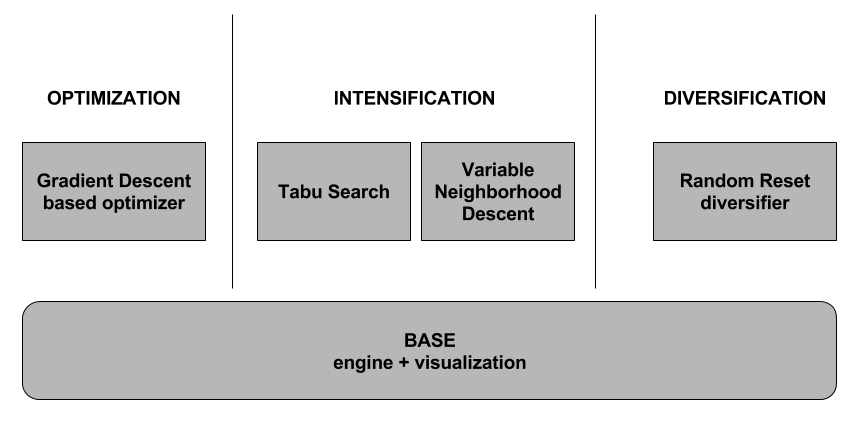
\includegraphics[scale=0.4]{/home/gw/Documents/wilbert/cs_master/courses/term1/datastructures_and_algorithms/cs_data_structures_and_algorithms/reports/img/img_code_structure.png}
	\caption{Description of the code structure}
	\label{fig:img_pecc}
\end{figure}

%% some figures %%%%%%%%%%%%%
As we can see, we have divided the three phases into modules, each one of them in charge of the related phase of the algorithm. All these modules share some functionality, which is enclosed in the BASE module. These modules are described as follows:

\begin{enumerate}
%%%%%
\item \textbf{Optimization module} \\
The optimization module is defined in the \textit{itsvnd/optimization/} folder and implements a gradient descent based optimizer ( see the \textit{LGradientDescentOptimizer.h} file ). We chose this optimizer instead of the LBFGS optimizer used in the paper. This optimizer is simpler than the LBFGS optimizer, but still yields good results, allowing to reach local minima in very few iterations and returning good configurations.
%%%%%
\item \textbf{Intensification module} \\
This module implements the metaheuristics of the paper. It is defined in the \textit{itsvnd/intensification/} folder, and implements \textit{Tabu-Search} ( \textit{LTSintensifier.h} file ) and \textit{Variable Neighborhood Descent} ( \textit{LVNDintensifier.h} file ). Both metaheuristics use the swap and insert neighborhoods, as opposed to the paper which only uses the insert neighborhood in the VND metaheuristic. This was decided becaused the intensifier yielded better results if both neighborhoods were used in both metaheuristics.
%%%%%
\item \textbf{Diversification module} \\
This module implements the random-reset strategy described in the paper. This module is defined in the \textit{itsvnd/diversification} folder ( \textit{LRRdiversifier.h} file ).
%%%%%
\item \textbf{Base module} \\
This is the core module, which implements the base functionality shared by the other modules, such as the configuration, circle, solver, etc. . This module is defined in the \textit{engine/} folder. There is also a visualization module written in Qt which is part of this module. We use this to visualize how well are our solutions, as we can see in figures 2 and 3.

\begin{figure}[H]
	\centering
	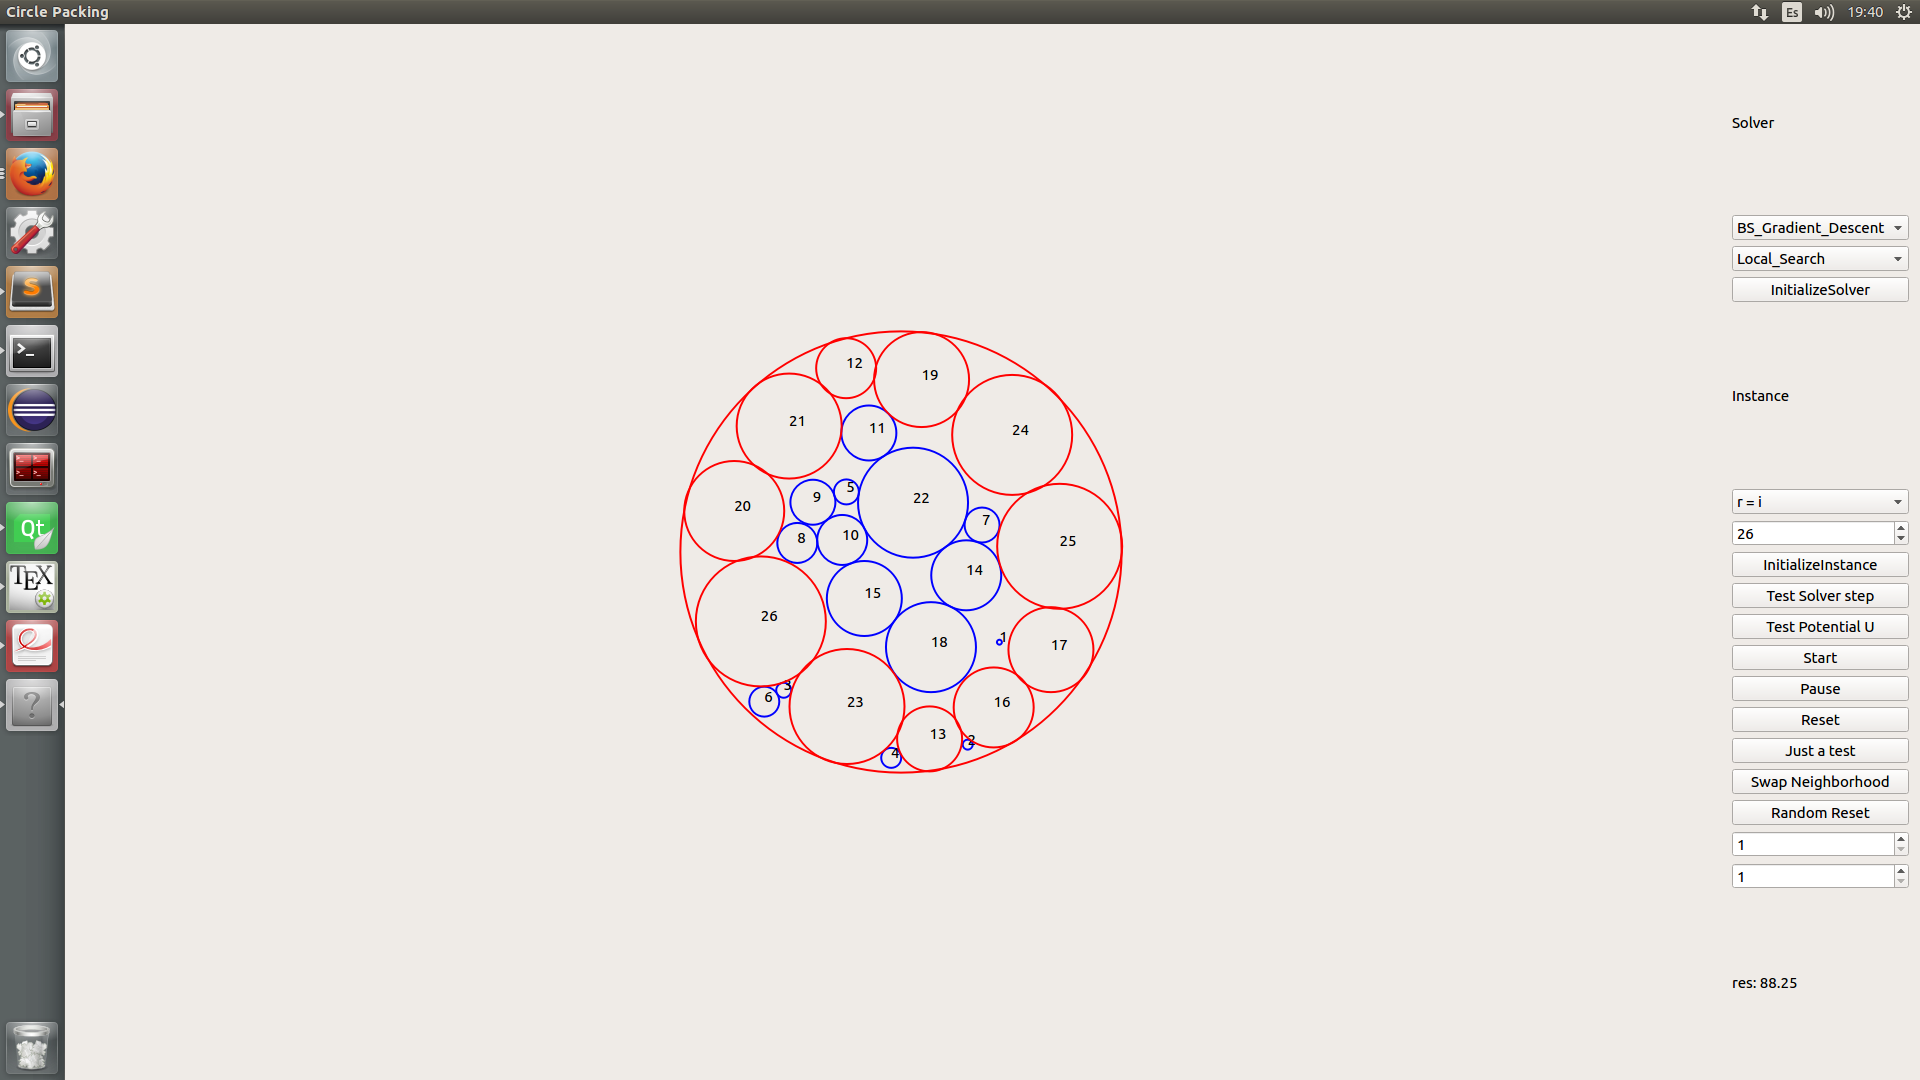
\includegraphics[scale=0.2]{/home/gw/Documents/wilbert/cs_master/courses/term1/datastructures_and_algorithms/cs_data_structures_and_algorithms/reports/img/img_feasible_sol.png}
	\caption{Qt based visualizer}
	\label{fig:img_pecc}
\end{figure}

\begin{figure}[H]
	\centering
	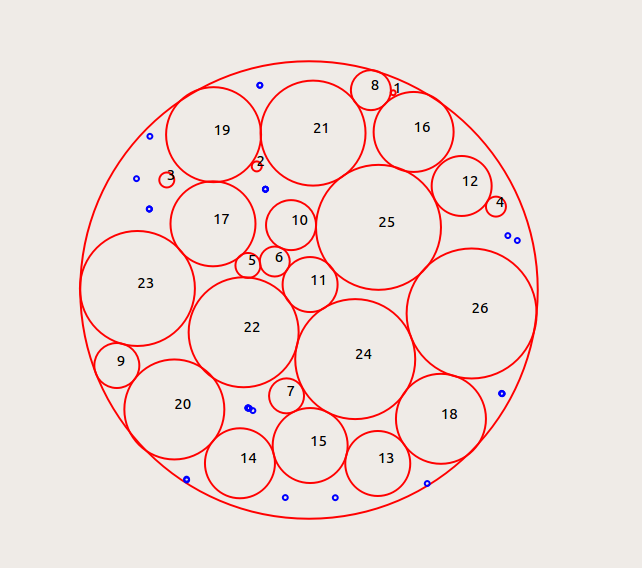
\includegraphics[scale=0.25]{/home/gw/Documents/wilbert/cs_master/courses/term1/datastructures_and_algorithms/cs_data_structures_and_algorithms/reports/img/img_vacant_points.png}
	\caption{Visualizer and vacant points for the insert neighborhood}
	\label{fig:img_pecc}
\end{figure}

\end{enumerate}

This describes all the code implemented for the project. The only part different than the paper is the optimizer, as described earlier.
%%%%%%%%%%%%%%%%%%%%%%%%%%%%%

%%%%%%%%%%%%%%%%%%%%%%%%%%%%%%%%%%%%%%%%%%%%%%%%%%%%%%%%%%%%%%%%%%%%%%%%%%%%%%%%%%%%%%%%%%%%%%%%%%%%%%%%%%%%%%%%%


\section{Plan for experimentation}\label{sec:solution}%%%%%%%%%%%%%%%%%%%%%%%%%%
%% Brief description of the solution %%%%%%%%%%%%%%%%%%
We have use as toy instance the \textit{r = i} instance. We have tested and the implemented method is off by a 7.5 percent from the results in the paper. We plan check for improvements in the algorithm and test it in the following way.

\begin{itemize}
\item Check with the \textit{r = i} instance for $n=[25-50]$ using only the optimizer to see how much can be achieved by optimization alone.
\item Check with the \textit{r = i} instance for $n=[25-50]$ using a basic implementation of a local search.
\item Check with the \textit{r = i} instance for $n=[25-50]$ using the Variable-Neighborhood-Descent method.
\item Check with the \textit{r = i} instance for $n=[25-50]$ using the Tabu-Search method.
\item Check with the \textit{r = i} instance for $n=[25-50]$ using the ITS-VND method.
\item Check with the $r=i,r=\sqrt{i},r=\frac{1}{\sqrt{i}}$ instances for $n=[25-50]$ using the ITS-VND method.
\item Check for improvements in the neighborhoods. Try to use a better neighborhood definition instead of the current swap and insert neighborhoods described in the paper.
\end{itemize}


%%%%%%%%%%%%%%%%%%%%%%%%%%%%%%%%%%%%%%%%%%%%%%%%%%%%%%%%%%%%%%%%%%%%%%%%%%%%%%%%%%%%%%%%%%%%%%%%%%%%%%%%%%%%%%%%%
\end{document}